\documentclass[12pt,a4j]{jarticle}
%\usepackage{graphicx}
\usepackage[dvipdfmx]{graphicx}
\begin{document}
\title{コンピュータリテラシレポート#12}
\author{1920031, 山川竜太郎}
\date{2019/07/12}
\maketitle


\section{課題の再掲}
演習3 自分が作成したWeb ページに関する説明をおこなうLaTeX 文書を作成しなさい。Webの画面を取り込むこと。また、Webページには演習1、演習2(の小課題)の内容、または以下のいずれか1つ以上が含まれること。

今回htmlページに盛り込んだ演習内容

/begin{itemize}
  /item (演習1)ページ内にリンクを作成する。
  /item (演習2)h1~h3を使って、CSSでデザインを調整する。
  /item (演習3)id機能使ってCSSを当てる。
  /item (演習3)箇条書きをする。
  /item (演習3)表を使ってみる。
/end{itemize}

\section{レポートの本文}

\section{何の目的で作るか}

ただのテストのような文章に対してCSSを当てるだけだと、デザインを行うのが非常に難しい。そこで基本情報技術者試験を受ける人向けに重要な単元を見せるという目的を立てた。ここにより「単元」が見出しの要素に当たるようになり、そこは見る人にとって意味を持つように目立たせる必要がある。つまり何の為にデザインを行うのか明確になる。

\section{どのように作るか}

h1の見出しはこのページのタイトルにしなくてはならない。「基本情報技試験の役立つメモ」にしておいた。CSSは、フォントを赤にした。また見出しには下に破線を引いて見出し項目であることを強調して、探したい項目を目で終えるようにする。全体的なレイアウトは全ての要素をmarginを用いて横に余白を設けてセンターに寄せるようにする。次の見出しは、「OSI参照モデル」について書く。これは箇条書きで列挙した方が理解しやすい内容なので、ulタグを使用する。またこのメモだけでは説明不十分な点を考慮して見出しに、OSI参照モデルの解説記事のリンクをaタグで貼る。また、箇条書きの項目にて、階層がいくつなのか強調させた方が閲覧者も意識が向くと思い、階層についてはbタグを使って文字を太くする。最後の見出しは「真偽表」を作成して、表形式にして視覚的に閲覧者に理解しやすいようにする。h1タグ以外の見出しのタグは、ページタイトルと各項目という感じに別れており、各項目の見出しについてはページタイトルより目立ってはいけないので、marginを使用して、若干横に余白を入れて見出し自体が小さくなるようにする。

\section{実際に作成したページ}

\begin{center}
  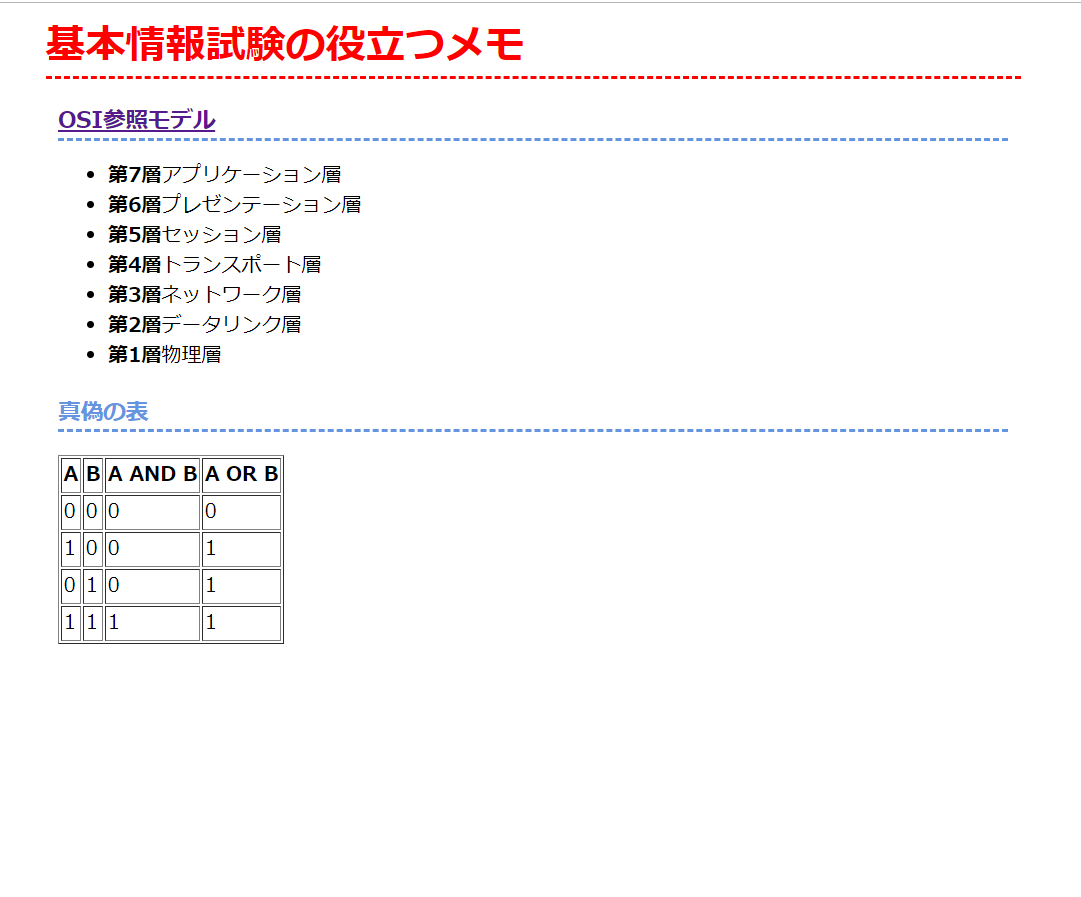
\includegraphics[width=10cm]{./index.png}
\end{center}

\section{考察}

まず、目的を持って作成したことにより、どのようなデザインを当てればいいのか明確になった。具体的には見出しのh1タグはフォントを他の見出しより大きくして、なおかつ色も目立つ色にしなければならないということだ。h2,h3はh1タグより目立ってしまうと閲覧者の意識が分散してしまい、ページビューした瞬間にどこを見て欲しいのかわからなくなってしまう。したがって、marginで幅をh1より抑えるとともに、fontも水色系にして落ち着かせた方が、ページビューした時にいきなりh2やh3に目がいってしまう確率を減らせる。「OSI参照モデル」について書いた項目は箇条書きを取り入れることによって、全ての項目が並列であることを閲覧者に指し示すように意識した。箇条書きの中で、別のタグを挟めるのか試してみたかったので、強調したかった部分にbタグを入れて太字にした。そうすることによって箇条書きの項目の中に太字とそうでないものが混在して表現できるようになった。「真偽の表」の表は、1行目にthタグを入れて表の見出しであることを強調したら、表の視覚効果が上げることができた。ページを作成する時に意識しなければならないのは、閲覧者にどこを最初にみて欲しいかということだ。強調してみて欲しいところはどこで、逆に優先度を落としてみて欲しい箇所は黒文字にして小さくする。そうすることによって閲覧者を誘導することができると言える。

\section{アンケート}

\subsection{Q1:HTMLによるページの記述はどれくらい知っていましたか。今回やってみてどうでしたか。}
やったことがあるので、だいたい知っていました。

\subsection{Q2:CSSによる表現の指定はどれくらい知っていましたか。今回やってみてどうでしたか。}
やったことがあるので、だいたい知っていました。

\subsection{Q3:リフレクション (今回の課題で分かったこと)・感想・要望をどうぞ。}
久々にhtmlを書いたので、結構楽しかったです。

\end{document}
